\Chapter{PLONGEMENTS VECTORIELS DE GRAPHES DE CONNAISSANCES}\label{chap:kge}

\section{Généralités}
\label{sec:kge-general}

\subsection{Introduction, notations et premiers concepts}
\label{subsec:kge-general-intro}

Les graphes de connaissance permettent d'appliquer des algorithmes de raisonnement très puissants. Toutefois, dans les bases de grande taille comme DBpédia ou Wikidata, la complexité en temps de ces algorithmes augmente rapidement, au point de les rendre inutilisables. Hors des algorithmes dédiés, les entités et les relations d'un graphe sont représentés de façon purement symbolique. La nécessité est donc apparue d'obtenir une représentation plus expressive des entités et relations d'un graphe. Pour ce faire, et suivant la dynamique du traitement automatique des langues, on a recours à des modèles de plongement. 

\todo{Reformuler, en partant des différents modes de représentation}

Un modèle de plongement est une méthode pour obtenir des représentations vectorielles denses et sémantiquement cohérentes des entités d'un graphe. Denses, c'est-à-dire de faible dimension, par opposition à une représentation sous forme de matrice d'adjacence $M(h) \in \{0, 1\}^{n_r \times n_e}$ où $M(h)_{i, j} = 1 \iff (h, r_i, e_j) \in \mathcal{KG}$. Sémantiquement cohérentes, car le modèle est construit de façon à envoyer une partie de l'information sémantique contenue dans le graphe vers l'espace vectoriel d'arrivé, afin que des entités sémantiquement proches dans le graphe aient des plongements vectoriels géométriquement proches.

Formellement, un modèle de plongement vectoriel est un modèle qui associe à chaque entité $e \in \mathcal{E}$ un vecteur $\mathbf{e} \in \mathbb{R}^d$, et à chaque relation $r \in \mathcal{R}$ un vecteur $\mathbf{r} \in \mathbb{R}^{d'}$. On note $\mathbf{E} = \{\mathbf{e}\}_{e \in \mathcal{E}} $ l'ensemble des plongements d'entité, $\mathbf{R} = \{\mathbf{r}\}_{r \in \mathcal{R}} $ l'ensemble des plongements de relation et $\Theta = (\mathbf{E}, \mathbf{R})$ l'ensemble des paramètres du modèle. Un modèle de plongement est caractérisé par $\Theta$ ainsi que par une fonction de score $\sigma_{\Theta} : \mathcal{E \times R \times E} \rightarrow [0, 1]$, définie sur l'ensemble des triplets possibles et paramétrée par $\Theta$.  

Pour entraîner un modèle de plongement, on a besoin d'un ensemble de triplets valides $\Delta_+$ (généralement, $\Delta_+ = \mathcal{KG}$), et un ensemble de triplets invalides $\Delta_-$. Comme un graphe ne contient, par construction, aucun triplet invalide, on construit $\Delta_-$ en fabriquant des triplets aléatoirement, et en supposant qu'ils sont invalides – c'est \textit{l'hypothèse du monde localement fermé}, empiriquement vérifiée dans n'importe quel graphe suffisamment grand.
\todo{Ajouter une ref à la section qui le justifie}

Une fois que l'on dispose de $\Delta_+$ et de $\Delta_-$, on peut commencer l'entraînement proprement dit. La procédure varie d'un modèle à l'autre, mais on en présente ici les grandes lignes. Tout d'abord, les paramètres (c'est-à-dire les plongements) sont initialisés aléatoirement. On définit une fonction de perte, typiquement une perte par marge maximale :
$$
J(\Theta) = \sum_{(h_+, r_+, t_+) \in \Delta_+} \sum_{(h_-, r_-, t_-) \in \Delta_-} \lfloor \gamma + \sigma_\Theta(h_+, r_+, t_+) - \sigma_\Theta(h_-, r_-, t_-) \rfloor
$$
On souhaite alors minimiser la perte. Pour cela, on calcule alors $\displaystyle \frac{\partial J}{\partial \Theta}$, et on met à jour $\Theta$ par descente de gradient. Il faut garder à l'esprit que mettre à jour $\Theta$ signifie mettre à jour les plongements vectoriels des entités et des relations du graphe, de façon à avoir un score maximal sur les triplets valides et minimal sur les triplets invalides. La procédure s'arrête une fois un critère de convergence atteint – par exemple, lorsque $J$ ne diminue plus.

Dans la suite de la section, on se propose de détailler plus avant les procédures communes à tous les modèles, et particulièrement la constitution des données d'entraînement, la distinction entre fonction de score et fonction d'énergie, ainsi que les fonctions de pertes communément utilisées. 

\section{Modèles de plongement}
\label{sec:kge-models}

\subsection{Modèles à translation : TransE et ses variantes}
\label{subsec:kge-models-transx}

On présente ici une première famille de modèles, les modèles \textit{à translation}, constituée de TransE et de ses dérivés. L'idée première de ces modèles consiste à représenter une relation entre deux entités comme une translation entre leurs plongements. Une relation $r$ est représentée par une translation $T_r$ de vecteur caractéristique $\mathbf{r}$ :
\begin{equation*}
    T_r : \mathbf{u} \mapsto \mathbf{u + r}
\end{equation*}

Un triplet $(h, r, t)$ est considéré comme valide si le plongement de $t$ est le translaté du plongement de $h$ par la translation $T_r$, c'est-à-dire $T_r(\mathbf{h}) = \mathbf{t}$. La plupart des modèles ajoutent une étape préalable à la translation : le plongement d'une entité $e$ est d'abord envoyé dans un nouvel espace, qui dépend de $r$ et éventuellement de $e$. Ensuite seulement, la translation a lieu dans ce nouvel espace.

Ainsi, on peut définir le cadre générale suivant pour décrire un modèle à translation :
\begin{itemize}
    \item une fonction de transformation $F_{e, r} : \mathbb{R}^d \rightarrow \mathbb{R}^{k}$
    \item une fonction d'énergie $E_\Theta(h, r, t) = \| F_{h, r}(\mathbf{h}) + \mathbf{r} - F_{t, r}(\mathbf{t}) \|_2 $
\end{itemize}

\subsubsection{TransE \cite{bordes2013translating}}
Le premier et le plus simple des modèles à translation, la fonction de transformation est la fonction identité ($\forall e, r, F_{e, r} = I_d$) – autrement dit, les plongements sont translatés directement, sans transformation préalable. En conséquence, les entités et les relations sont plongées dans le même espace $\mathbb{R}^d$, et la fonction d'énergie est donc
\begin{equation}
    E_\Theta(h, r, t) = \| \mathbf{h + r - t} \|_2
    \label{eq:transe-main}
\end{equation}

Le nombre de paramètres est donc $d \times (N + M)$, linéaire en le nombre d'éléments du graphe. 

La force de TransE réside dans sa simplicité théorique et son faible nombre de paramètres. Toutefois, cette simplicité se paye par une faible expressivité, qui limite sa capacité à modéliser des relations autres que \textit{one-to-one} :
\begin{itemize}
    \item relation \textit{many-to-one} : si plusieurs entités $h_1, h_2, \ldots, h_k$ sont reliées à une même entité $t$ par une relation $r$, alors les translatés $\mathbf{h_i + r}$ doivent tous être égaux, donc $\mathbf{h_1  = h_2 = \ldots = h_k}$;
    \item relation \textit{one-to-many} : comme au-dessus, si $h$ est lié par $r$ à plusieurs entités $t_1, \ldots, t_k$, alors nécessairement $\mathbf{t_1 = t_2 = \ldots = t_k}$;
    \item relations symétriques : si $r$ est symétrique, c'est-à-dire $h  \overset{r} \rightarrow t \implies t   \overset{r} \rightarrow h$, alors la translation de la translation par $r$ doit donner l'élément de départ, donc $\mathbf{r} = 0$
\end{itemize}

\subsubsection{TransH \cite{fu2014learning}}

\begin{figure}[hbt]
    \centering
    \begin{tikzpicture}
\def\rep{3};
\def\size{1};
\def\px{-0.5*\size};
\def\py{1.5*\size};
\def\pz{-.5*\size};
\def\hplane{(\px, \py, \pz)};

\def\hsize{2};
\def\vsize{2};
\def\offset{0.5};

\tikzmath{
    \base=2;
    \rx=1*\base;
    \ry=0.5*\base;
    \rz=0.5*\base;
    % h_p
    \hp1=-0.5;
    \hp2=0.5;
    \hp3=-(\hp1*\rx+\hp2*\ry)/\rz;
    \h1=\hp1+\rx;
    \h2=\hp2+\ry;
    \h3=\hp3+\rz;
    % t_p
    \tp1=0.5;
    \tp2=1;
    \tp3=-(\tp1*\rx+\tp2*\ry)/\rz;
    \t1=\tp1+\rx;
    \t2=\tp2+\ry;
    \t3=\tp3+\rz;
    % v
    \v1=-sqrt(((\rx)^2) / ((\rx)^2 + (\rz)^2));
    \v2=0;
    \v3=sqrt(((\rz)^2) / ((\rx)^2 + (\rz)^2));
    % u
    \u1=-\ry / (\rx - (\v1 * \rz) / \v3);
    \u2=1;
    \u3=-\u1*\v1/\v3;
}

\newcommand{\makeplane}{
    % Make axis
    \node (o) at (0, 0, 0) {};
    \node (x) at (\rep, 0, 0) {};
    \node (y) at (0, \rep, 0) {};
    \node (z) at (0, 0, \rep) {};
    
    \draw[axis] (o.center) -- (x);
    \draw[axis] (o.center) -- (y);
    \draw[axis] (o.center) -- (z);
    
    % Make plane
    \filldraw[plane] 
    (\hsize*\v1, \hsize*\v2, \hsize*\v3)
    --  ++(\vsize*\u1, \vsize*\u2, \vsize*\u3)
    -- ++(-2*\hsize*\v1, -2*\hsize*\v2, -2*\hsize*\v3)
    -- ++(-\vsize*\u1, -\vsize*\u2, -\vsize*\u3)
    -- node[below, accent1, sloped, near end] {$H_r$} cycle;
}

\begin{scope}
    % Make axis
    \makeplane
    
    \node[node=accent1, label={[accent1]$\bf{h_\bot}$}] (hp) at (\hp1,\hp2,\hp3) {};
    \node[node=black, label={$\bf{h}$}] (h) at (\h1,\h2,\h3) {};
    \draw[accent1, thick, ->] (h) -- (hp);
    
    \node[node=accent1, label={[accent1]$\bf{t_\bot}$}] (tp) at (\tp1,\tp2,\tp3) {};
    \node[node=black, label={$\bf{t}$}] (t) at (\t1,\t2,\t3) {};
    \draw[accent1, thick, ->] (t) -- (tp);
\end{scope}

\begin{scope}[xshift=7.5cm]
    % Make axis
    \makeplane
    
    \node[node=black, label={$\bf{h_\bot}$}] (hp) at (\hp1,\hp2,\hp3) {};
    % \node[node=gray, label={$h$}] (h) at (\h1,\h2,\h3) {};
    % \draw[gray, thin, ->] (h) -- (hp);
    
    \node[node=black, label={$\bf{t_\bot}$}] (tp) at (\tp1,\tp2,\tp3) {};
    % \node[node=gray, label={$t$}] (t) at (\t1,\t2,\t3) {};
    % \draw[gray, thin, ->] (t) -- (tp);
    
    \node (hr) at (\tp1-\offset*\u1,\tp2-\offset*\u2,\tp3-\offset*\u3) {};
    
    \draw[accent1, thick, ->] (hp) -- node[sloped, below] {$\bf{r}$} (hr.center);
    \draw[thin, accent2, <->] (hr.center) -- node[accent2, near start,right] {$E(h, r, t)$} (tp);
\end{scope}
\end{tikzpicture}
    \caption[Principe général de TransH]{Principe général de TransH : pour calculer le score d'un triplet $(h, r, t)$, on commence par projeter $\bf{h}$ et $\bf{t}$ sur l'hyperplan $H_r$, puis on translate $\bf{h}$. Le score du triplet est égal à la distance entre le translaté de $\bf{h}$ et $\bf{t}$.}
    \label{fig:transh}
\end{figure}

\begin{figure}[hbt]
    \centering
    \begin{tikzpicture}
[
scale=0.8,
separation/.style={-, draw=gray!40, dashed},
proja/.style={-, draw=red!20, thin},
projb/.style={-, draw=blue!20}
]

\node  (0) at (0, 0) {};
\node (1) at (0, 2) {};
\node (2) at (2, 3) {};
\node (3) at (4, 4) {};
\node (4) at (3, -1) {};
\node (5) at (3, 1) {};
\node (6) at (7, 3) {};
\node (7) at (7, 1) {};
\node (8) at (4, 2) {};
\node (9) at (4, -2) {};
\node (10) at (7, -3) {};
\node (11) at (3, -5) {};
\node (12) at (0, -4) {};
\node (13) at (-2, 4) {};
\node (14) at (-2, 6) {};
\node (15) at (-6, 2) {};
\node (16) at (-6, 4) {};
%\node (17) at (3, -8) {};
\node (18) at (7, -6) {};
\node (19) at (9, -4.75) {};
\node (20) at (0, -7) {};
\node (21) at (-4, -5) {};
\node (22) at (-8, -2.75) {};
\node (23) at (-8, 6) {};
\node (24) at (-4, 8) {};
\node (25) at (0, 8) {};
\node (26) at (0, 4) {};
\node (27) at (-8, -4) {};
\node (28) at (-9.5, -3.5) {};
\node (29) at (-13, 1) {};
\node (30) at (-8, -4.75) {};
\node (31) at (-7.1, -4.35) {};
\node (32) at (-2, -1) {};
\node (45) at (5, -7) {};
\node (46) at (9, -2.75) {};

\fill [plane-content=accent2] (27.center) -- (23.center) -- (24.center) -- (25.center) -- (26.center) -- (0,0) -- (32.center) -- cycle;
\fill [plane-content=accent2] (27.center) -- (30.center) -- (31.center) -- cycle;
\fill [plane-content=accent1] (0,0) -- (46.center) -- (19.center) -- (18.center) -- (45.center) -- (20.center) -- (27.center) -- cycle;
\fill [plane-content=accent1] (27.center) -- (28.center) -- (22.center) -- cycle;
\fill[white, path fading=fade out] (0,0) circle (3);
\fill[white, path fading=fade out] (3, 1) circle (5);
    
\node [node=accent2, label={270:Sean McBride}] (33) at (-6, 4) {};
\node [node=accent2, label={Paris}] (34) at (-2, 6) {};
\node [node=accent2, label={Dublin}] (35) at (-2, 4) {};
\node [node=accent2, label={270:Oscar Wilde}] (36) at (-6, 2) {};
\node [node=accent1, label={200:Oscar Wilde}] (37) at (0, -4) {};
\node [node=accent1, label={Paris}] (38) at (4, -2) {};
\node [node=accent1, label={200:Sean McBride}] (39) at (3, -5) {};
\node [node=accent1, label={Dublin}] (40) at (7, -3) {};
\node [node, label={Sean McBride}] (41) at (3, 1) {};
\node [node, label={Oscar Wilde}] (42) at (0, 0) {};
\node [node, label={Paris}] (43) at (4, 4) {};
\node [node, label={Dublin}] (44) at (7, 1) {};

\draw [plane-border=accent2] (22.center) to node [above, sloped] {Hyperplan \texttt{dbo:birthPlace}} (23.center);
\draw [plane-border=accent2] (23.center) to (24.center);
\draw [plane-border=accent2] (25.center) to (26.center);
\draw [plane-border=accent1] (19.center) to (45.center);
\draw [plane-border=accent1] (27.center) to node [above, sloped] {Hyperplan \texttt{dbo:deathPlace}} (20.center);
\draw [plane-border=accent2] (22.center) to (27.center);
\draw [plane-border=accent1] (28.center) to (27.center);
\draw [plane-border=accent1] (28.center) to (22.center);
\draw [plane-border=accent2] (27.center) to (30.center);
\draw [plane-border=accent2] (30.center) to (31.center);
\draw [vec=accent1] (12) to (9);
\draw [vec=accent1] (11) to node[below, sloped]{\footnotesize \texttt{dbo:deathPlace}} (10);
\draw [vec=accent2] (16) to node[above, sloped]{\footnotesize \texttt{dbo:birthPlace}} (14);
\draw [vec=accent2] (15) to (13);
\draw [style=proja] (0.center) to (12.center);
\draw [style=proja] (5.center) to (11.center);
\draw [style=proja] (7.center) to (10.center);
\draw [style=proja] (3.center) to (9.center);
\draw [style=projb] (0.center) to (15.center);
\draw [style=projb] (5.center) to (16.center);
\draw [style=projb] (3.center) to (14.center);
\draw [style=projb] (7.center) to (13.center);
\draw [style=separation] (27.center) to (32.center);
\end{tikzpicture}
    \caption[Exemple des possibilités laissées par TransH]{Exemple de deux relations \texttt{dbo:birthPlace} et \texttt{dbo:deathPlace}, ainsi que leurs hyperplans associés.}
    \label{fig:transh-dual}
\end{figure}

\subsubsection{TransD}

TransD est une extension de TransE dans laquelle les entités à translater sont transformées via une fonction de transformation linéaire qui dépend à la fois de la relation considérée et de l'entité à transformer. Outre les plongements usuels $\bf{e}, \bf{r}$ définis pour chaque entité $e \in \Ent $ et chaque relation $r \in \Rel$, le modèle TransD entraîne aussi des vecteurs de projection $\bf{e_p}$ et $\bf{r_p}$. Ces vecteurs servent à construire dynamiquement une matrice de tranformation $M_{e, r}$:
\begin{equation}
    \label{eq:kge-transd-matrix}
    \bf{M}_{e, r} = \bf{r_p \cdot e_p^\top + I_{d' \times d}}
\end{equation}
% TODO: indices sont gras ou pas ?

La fonction de transformation pour une entité $e$ et un triplet $r$ s'écrit alors :
\begin{equation}
    \label{eq:kge-transd-function}
    F_{e, r} = \bf{M}_{e, r} \cdot \bf{e}
\end{equation}

Soit finalement une fonction d'énergie :
\begin{equation}
    E_\Theta(h, r, t) = \| (\bf{r_p \cdot h_p^\top + I_{d' \times d}}) \cdot \bf{h} + \mathbf{r} - (\bf{r_p \cdot t_p^\top + I_{d' \times d}}) \cdot \bf{t} \|_2 
\end{equation}
On peut voir cette équation comme l'équation de TransE avec un terme correcteur :
\begin{equation}
    E_\Theta(h, r, t) = \| (\bf{h + r - t}) + \bf{r_p} \cdot (\bf{ h_p^\top \cdot h - t_p^\top \cdot t}) \|_2 
\end{equation}


\subsubsection{Autres modèles}

\subsubsection{Résumé}


\begin{table}[ht]
\caption{Propriétés de quelques modèles à translation}
\centering
\begin{tabular}{|c|c|c|c|c|}
\hline\rowcolor[gray]{0.8}\color{black}
Modèle & Entités & Relations & Transformation & Nombre de paramètres\\\hline
TransE & $\mathbf{e} \in \mathbb{R}^d$ & $\mathbf{r} \in \mathbb{R}^d$ & Aucune & $d \times (M + N)$ \\
TransH & $\mathbf{e} \in \mathbb{R}^d$ & $\mathbf{r, n_r} \in \mathbb{R}^d$ & Projection sur un hyperplan & $d \times (2M + N)$ \\
TransD & $\mathbf{e, e_p} \in \mathbb{R}^d$ & $\mathbf{r, r_p} \in \mathbb{R}^d$  & Transformation linéaire & $2d \times (M + N)$ \\\hline
\end{tabular}
\label{tab:transx}
\end{table}

\subsection{Modèles multiplicatifs : RESCAL et ses variantes}
\label{subsec:kge-models-mult}

\subsubsection{RESCAL}
Soit un graphe $\KG$, représenté sous la forme d'un tenseur d'adjacence $\mathcal{T} \in \{0, 1\}^{N \times M \times N}$. Pour une relation $r \in \mathcal{R}$ donnée, on dispose d'une matrice d'adjacence $M^r$, de dimension $N \times N$, telle que $M_{i, j}^r$ vaut $1$ si $e_i$ est lié à $e_j$ par la relation $r$, et $0$ sinon.

\ldots

Le modèle RESCAL \cite{nickel2011learning} construit donc un plongement vectoriel $\mathbf{e}$ de dimension $d$ pour chaque entité $e \in \mathcal{E}$, et une matrice $W_r$ de dimension $n \times n$ pour chaque relation $r \in \mathcal{R}$. La fonction de score d'un triplet s'écrit :
\begin{equation}
    \sigma(h, r, t) = \mathbf{h^\top \cdot W_r \cdot t}
    \label{eq:rescal}
\end{equation}

Notons $w_{i, j}$ la coordonnée $i,j$ de $W_r$, on peut réécrire l'équation~\ref{eq:rescal} sous la forme~:

\begin{equation}
    \sigma(h, r, t) = \sum_{i, j = 1}^{d} \mathbf{h_i \cdot t_j} \cdot w_{i, j}
\end{equation}

Ainsi, toutes les combinaisons $\mathbf{h_i t_j}$ de $\mathbf{h}$ et de $\mathbf{t}$ apparaissent dans la fonction de score, avec un coefficient $w_{i, j}$. En ce sens, RESCAL propose une expressivité maximale et permet de modéliser une large palette de relations. Par exemple, si $\mathbf{W_r}$ est symétrique (c'est-à-dire, $\mathbf{W_r} = \mathbf{W_r}^\top$), on a $w_{i,j} = w_{j, i}$ pour tous $i, j = 1, \ldots, d$, et donc :

\begin{equation}
    \sigma(h, r, t) = \sum_{i, j = 1}^{d} \mathbf{h_i \cdot t_j} \cdot d_{i, j}
    =  \sum_{i, j = 1}^{d} \mathbf{h_j \cdot t_i} \cdot w_{j, i}
    =  \sum_{i, j = 1}^{d} \mathbf{h_j \cdot t_i} \cdot w_{i, j}
    = \sigma(t, r, h)
\end{equation}

Une matrice symétrique induit donc une fonction de score symétrique elle aussi; cela permet de modéliser des relations symétriques. Inversement, si $\mathbf{W_r}$ est antisymétrique (c'est-à-dire, $\mathbf{W_r} = -\mathbf{W_r}^\top$), on aura une fonction de score antisymétrique, ce qui permet de modéliser une relation antisymétrique.

Cette expressivité se paie toutefois par un nombre plus élevé de paramètres ($d^2$ par relation, contre $d$ pour TransE); au-delà des considérations de mémoire, l'entraînement de ces $d^2$ paramètres est plus difficile et la convergence plus lente.

\subsubsection{DistMult}

DistMult \cite{distmult} vise à simplifier RESCAL pour le rendre plus facile à entraîner et moins sujet au surapprentissage. Pour cela, on garde la fonction de score de RESCAL, exprimée dans l'équation~\ref{eq:rescal}, mais on impose que la matrice $\mathbf{W_r}$ soit diagonale – soit $d$ paramètres par relation, comme TransE, au lieu de $d^2$. Cela revient à représenter une relation $r$ par un vecteur $\mathbf{r}$ de dimension $d$, et à poser $\mathbf{W_r = I_{d\times d} \cdot r}$. La fonction de score s'écrit donc :
\begin{equation}
    \label{eq:distmult}
    \sigma(h, r, t) = \mathbf{h^\top \cdot I_{d\times d}r \cdot t}
\end{equation}

Ce qui se réécrit:
\begin{equation}
    \sigma(h, r, t) = \sum_{i=1}^{d} \mathbf{h_i r_i t_i}
\end{equation}

Ainsi, la fonction de score peut être vue comme un produit scalaire à trois vecteurs. Comparé à RESCAL, l'expressivité est très réduite : seule les combinaisons de la forme $\mathbf{h_i t_i}$ sont utilisées pour le calcul du score. De plus, $\sigma$ est toujours symétrique, donc le sujet et l'objet d'un triplet ne sont pas différenciés.

\subsubsection{ComplEx}
\label{subsec:complex}

ComplEx est une extension de DistMult dans l'espace complexe. Comme RESCAL, il s'appuie sur une décomposition de la matrice d'adjacence $\bf{X}_r$ associée à la relation $r$ pour en réduire la dimension; toutefois, au lieu d'utiliser la décomposition en valeurs singulières (SVD), il repose sur la décomposition en valeurs propres. Selon le théorème spectral, tout matrice normale est diagonalisable sur une base orthonormale :
\begin{equation}
    \bf{X}_r = \bf{E \cdot W_r \cdot \compconj{E}^\top}
\end{equation}
Avec $\bf{W}_r \in \mathbb{C}^{|\Ent| \times |\Ent|}$ une matrice diagonale. En gardant alors les $d \times d$ premières coordonnées de $\bf{W}_r$ pour former les matrices $\bf{W}_r^{(d)} \in \mathbb{C}^{d \times d}$ et $\bf{E}^{(d)} \in \mathbb{C}^{|\Ent| \times d}$, on obtient une approximation de $\bf{X}_r$ de dimension $d$ :
\begin{equation}
    \bf{X}_r \approx \bf{E}^{(d)} \cdot \bf{W}_r^{(d)} \cdot \compconj{ \bf{E}^{(d)}}^\top
\end{equation}

Enfin, la matrice devant être réelle, son approximation en basse dimension est projetée dans $\R$ en ne considérant que la partie réelle de $\bf{E}^{(d)} \cdot \bf{W}_r^{(d)} \cdot \compconj{ \bf{E}^{(d)}}^\top$. Autrement dit, la fonction de score de ComplEx peut s'écrire :
\begin{equation}
    \sigma(h, r, t) = \Re(\bf{h^\top \cdot W}_r \cdot \compconj{\bf{t}})
\end{equation}
Avec $\bf{h, t} \in \mathbb{C}^d$ des vecteurs complexes, et $\bf{W}_r$ une matrice complexe diagonale de dimension $d \times d$.

Un avantage théorique de la fonction de score de ComplEx par rapport aux précédentes est qu'elle est capable d'être symétrique, antisymétrique ou ni l'un ni l'autre, selon la position de $\bf{W}_r$ dans l'espace complexe. Considérons d'abord le cas où $\bf{W}_r$ est réelle ($\bf{W}_r \in \R^{d \times d}$). On a :
\begin{align}
    \sigma(h, r, t) &= \Re(\bf{h^\top \cdot W}_r \cdot \compconj{\bf{t}}) \\
    &= \Re\left((\compconj{\bf{h^\top \cdot W}_r \cdot \compconj{\bf{t}}})^\top\right) \label{eq:complex-symmetric-1} \\
    &= \Re\left( \compconj{\compconj{\bf{t}}^\top \cdot \compconj{\bf{W}_r}^\top \cdot 
    \compconj{\bf{h^\top}}^\top}\right) \label{eq:complex-symmetric-2} \\
    &= \Re\left(\bf{t}^\top \cdot \bf{W}_r \cdot \compconj{\bf{h}}\right) \label{eq:complex-symmetric-3} \\
    &= \sigma(t, r, h)
\end{align}
\ref{eq:complex-symmetric-1} est vraie car la partie réelle est invariante par conjugaison, et \ref{eq:complex-symmetric-3} parce que $\bf{W}_r$ est réelle et symétrique. Ainsi, la fonction de score est symétrique lorsque le plongement de la relation associée est réel, on peut donc modéliser plus fidèlement une relation symétrique. Si un triplet $(h, r, t)$ est valide et présent à l'entraînement, le modèle sera entraîné pour maximiser $\sigma(h, r, t)$; or, sous réserve que $\bf{W}_r$ soit réelle, on aura $\sigma(t, r, h) = \sigma(h, r, t)$ et donc on aura bien l'équivalence : $(h, r, t) \text{ est valide} \iff (t, r, h) \text{ est valide}$.

Inversement, si $\bf{W}_r$ est imaginaire pure, c'est-à-dire $\bf{W}_r \in i\R$, on aura $\compconj{\bf{W}_r} = - \bf{W}_r$; en injectant ce résultat dans l'équation \ref{eq:complex-symmetric-2}, on aura :
\begin{equation}
    \sigma(h, r, t) = - \sigma(t, r, h)
\end{equation}
Soit une fonction de score antisymétrique. Donc un plongement imaginaire pur modélisera des relations antisymétriques, puisqu'un score élevé pour le triplet $(h, r, t)$ impliquera nécessairement un score faible pour le symétrique $(t, r, h)$.

Enfin, dans le cas général où $\bf{W}_r$ n'est ni réelle, ni imaginaire pure, la relation $r$ modélisée ne sera ni symétrique, ni antisymétrique. Évidemment, il s'agit là de propriétés \textit{théoriques} du modèle : en particulier, ces propriétés ne sont utiles qu'à la condition que le modèle soit capable de faire converger les plongements des relations symétriques vers l'espace réel, et les plongements des relations antisymétriques vers l'espace des imaginaires purs. Toutefois, cela indique une expressivité \textit{a priori}, que n'ont ni TransE, ni DistMult. En effet, pour TransE, une relation symétrique devrait vérifier $\bf{h + r - t} \approx 0$ et $\bf{t + r - h} \approx 0$, pour tous les plongements $\bf{h, t}$; en injectant la seconde équation dans la première, on obtient $\bf{h + r + r} \approx h, \forall \bf{h}$, soit $\bf{r \approx -r}$ et donc $\bf{r} \approx 0$. Ainsi,  une relation modélisée par TransE n'est pas symétrique, sauf dans le cas particulier où $\bf{r}$ est nul. Dans le cas de DistMult, toutes les relations sont symétriques.

\subsection{Autres modèles}
\label{subsec:kge-models-misc}

\subsubsection{RDF2Vec}

Le modèle RDF2Vec s'inspire du modèle de plongement Word2Vec, très utilisé pour produire des plongements lexicaux.

Il fonctionne en deux étapes : d'abord, des chemins sont prélevés dans le graphe de connaissance au moyen de marches aléatoires – ces chemins sont simplement des suites d'entités et de relations connectés entre eux.

% Ajouter l'équation pour définir une marche aléatoire

Ensuite, ces chemins sont passés en entrée à un réseau de neurones : le but de ce réseau est de prédire une entité en fonction des plongements de son contexte, ou au contraire de prédire le contexte d'une entité à partir du plongement de celle-ci.

\todo{ajouter des détails, notamment les équations du réseau, et les différents modes de sampling des random walks + figure}

\subsubsection{\textit{Graph Convolutional Networks}}
\subsubsection{Modèles hyperboliques}


\section{Séparabilités des plongements vectoriels}

Puisque le but général de ce travail est d'identifier des groupes sémantiquement cohérents d'entités à partir de leur proximité géométrique, il nous est nécessaire d'évaluer la capacité d'un modèle à plonger les instances d'une même classe dans la même région de l'espace euclidien. On formalise cette exigence en définissant une tâche de séparabilité, dont le but est de mesurer si des groupes d'entités appartenant à deux classes différentes sont linéairement séparables.

Le principe général est le suivant : pour deux classes $A$ et $B$, on prélève aléatoirement $N$ instances de $A$ et $N$ instances de $B$; on attribue aux instances de $A$ l'étiquette $0$ et à celles de $B$ l'étiquette $1$. Le résultat est un jeu de données $D = \{\mathbf{e_i}, y_i \}_{i=1, \ldots, 2N}$, avec $\bf{e}_i \in \R^d$ le plongement vectoriel de l'entité $e_i$, et $y_i \in \{ 0, 1\}$ l'étiquette associée à $e_i$. On entraîne alors une SVM linéaire sur 75\% de ces points, et on prédit ensuite les étiquettes des 25\% restant. Les étiquettes prédites peuvent alors êtres prédites aux étiquettes d'origine, selon les mesures usueles de la classification automatique : précision, rappel, mesure $F1$. Dans nos expériences, on choisit $N=1000$; si une classe possède moins que ces $N$ instances, on utilise toutes les instances de cette classe.


La difficulté qu'il y a à séparer une classe $A$ d'une classe $B$ dépends beaucoup de $A$ et de $B$ : intuitivement, il est plus difficile de distinguer un \dbo{College} d'une \dbo{University} qu'un \dbo{Aircraft} d'une \dbo{Person}. De plus, on peut imaginer que la taille de la classe (c'est-à-dire le nombre d'instances qui en font partie) influe aussi sur la difficulté, comme c'est souvent le cas en apprentissage automatique. Nous avons donc mis au point trois métriques pour évaluer la difficulté \textit{a priori} de la tâche de séparation pour toute paire de classe $(A, B)$. La première de ces métriques est la distance lexicale entre les classes, mesurée grâce à des plongements lexicaux; la deuxième est une distance taxonomique entre les classes, basée sur la distance entre les classes dans l'arbre; la troisième est un indicateur de la fréquence des deux classes dans la base de connaissance.

\subsubsection{Distance lexicale}

La première de nos métriques est une distance entre les classes, basée sur la proximité sémantique des noms de ces classes. Pour une classe $X$ quelconque, on commence par séparer les mots qui composent son URI : dans DBpédia, la convention de nommage pour les classes est le \textit{CamelCase}, donc l'entité \texttt{SportsTeamMember} est séparée en \texttt{"sports"}, \texttt{"team"} et \texttt{"member"}. On utilise alors des plongements lexicaux pour représenter chacun de ces mots par un vecteur de $\R^d$, et on moyenne ensuite ces vecteurs pour obtenir une représentation vectorielle $\mathbf{X}$ de la classe $X$ de départ. On peut alors définir la distance entre deux classes $A$ et $B$ comme la distance euclidienne entre leurs représentants :
\begin{equation}
d_\text{lex}(A, B) = \| \mathbf{A} - \mathbf{B} \|_2
\end{equation}

%\footnote{We used word embeddings from \href{https://fasttext.cc/docs/en/english-vectors.html}{https://fasttext.cc/docs/en/english-vectors.html}, trained on Common Crawl \cite{mikolov2018advances}} 

\subsubsection{Distance taxonomique}
On introduit également une distance entre les classes basée sur leur distance dans la taxonomie de départ. Puisqu'une taxonomie est un arbre, il existe un unique chemin (non-orienté) de longueur minimale entre n'importe quelle paire de classes $A$ et $B$ dans la taxonomie. En effet, un arbre est un graphe connexe minimal : connexe, donc au moins un chemin existe entre $A$ et $B$; minimal, donc il ne peut exister qu'un chemin, sinon on pourrait supprimer une arête d'un des deux chemins sans perdre la connexité, ce qui contredirait la minimalité du graphe. On note donc $\text{path}(A, B) = \{(A \rightarrow c_1), (c_1 \rightarrow c_2), \ldots, (c_k \rightarrow B)\}$ ce chemin. Pour une arête $e = (c_i \rightarrow c_j)$ donnée, on définit également sa profondeur $\text{depth}(e)$ comme le nombre d'arêtes entre elle et la racine de l'arbre : une arête connectée directement à la racine a une profondeur nulle; une arête connectée à un successeur immédiat de la racine a une profondeur égale à $1$, etc.
On peut alors définir la distance taxonomique comme :
\begin{equation}
    d_\text{tax}(A, B) = \sum_{e \in \text{path}(A, B)} \frac{1}{\displaystyle 2^{\text{depth}(e)}}
\end{equation}
Cette distance taxonomique est la longueur du chemin entre $A$ et $B$, pondérée par la profondeur des arêtes qui composent ce chemin. Le poids d'une arête est $1/2^{\text{depth}(e)}$ et diminue donc avec sa profondeur : en effet, dans une taxonomie, la profondeur d'une arête est un indicateur de la spécificité de l'axiome de subsumption associé à cette arête. Les axiomes associés aux arêtes de profondeur $0$ sont des axiomes très généraux, comme par exemple $\dbo{Place} \sqsubseteq \texttt{owl:Thing}$ («un endroit est une chose») ou $\dbo{Agent} \sqsubseteq \texttt{owl:Thing}$ («un agent est une chose»). À la profondeur $1$, les axiomes sont déjà plus précis – par exemple, $\dbo{Person}\sqsubseteq \dbo{Agent}$ («une personne est un agent»). À des profondeurs plus élevés, les axiomes deviennent très spécifiques, comme par exemple $\dbo{MotorRace} \sqsubseteq \dbo{Race}$ à la profondeur $4$. Aussi, deux classes séparées par une arête de faible profondeur sont plus sémantiquement plus distantes que deux classes séparées par une arête de profondeur élevée.

Quant au choix d'une décroissance spécifiquement égale à $\frac{1}{2^k}$, il permet à notre distance d'avoir une propriété intéressante : une classe $A$ est plus proche de ses sous-classes que de n'importe quelle autre classe. Vérifions-le en prenant $A$ une classe de profondeur $d$, et $A'$ une sous-classe de $A$ de profondeur $d' > d$. Alors la distance entre $A$ et $A'$ s'écrit :
\begin{align*}
    d_\text{tax}(A, A') &= \sum_{k = d}^{d'} 2^{-k} \\
    &= 2^{-d} \cdot \sum_{k=0}^{d'-d} 2^{-k} \\
    &= 2^{-d} (2^{d'-d} - 1) % À vérifier
\end{align*}
Or la distance entre $A$ et sa superclasse immédiate $B$ est 
\begin{align*}
    d_\text{tax}(A, B) &= 2^{-(d-1)} \\
\end{align*}
\todo{ajouter les équations correctes pour la distance taxonomique}

\subsubsection{Influence de la fréquence}

Une entité $e$ impliquée dans de nombreux triplets sera vue plus souvent pendant la phase d'entraînement, et aura donc un plongement vectoriel plus fiable. Comme ce plongement vectoriel dépend à son tour des plongements des entités et des relations qui sont connectée à $e$, il est possible que les entités appartenant à des classes rares soient impliqués dans des relations rares elles-aussi et connectées à des entités rares; cela produirait des plongements vectoriels moins fiable que la moyenne. Pour vérifier cette hypothèse, on évalue également l'influence de l'effectif des classes (\textit{i.e.} le nombre d'instances qui appartiennent à cette classe) sur les scores de séparabilité. Pour obtenir une mesure synthétique de la fréquence d'une paire de classe $(A, B)$, on utilise la moyenne harmonique des fréquences de $A$ et de $B$. L'utilisation de la moyenne harmonique plutôt que de la moyenne arithmétique usuelle permet de mieux refléter les déséquilibres entre les fréquences de $A$ et de $B$ : si $N_A$ est la fréquence de la classe $A$ et $N_B$ celle de la classe $B$, et que $N_A$ est supérieur à $N_B$ d'un ordre de grandeur, alors la moyenne arithmétique de $N_A$ et $N_B$ a le même ordre de grandeur que $N_A$, et n'indique donc pas que $B$ est rare par rapport à $A$.

\subsection{Résultats}

On évalue six modèles de plongement sur la tâche de séparabilité : TransE, TransH, TransD, DistMult, ComplEx, RDF2Vec. La séparabilité est calculée sur 10 000 paires de classes issues de DBpédia. On donne les scores de séparabilité moyens pour chaque modèle dans le tableau \ref{tab:separability-results}; on aggrège également les résultats pour différentes valeurs de distance lexicale et taxonomique dans la figure \ref{fig:separability-lexical}, et pour différentes fréquences de classes dans la figure \ref{fig:separability-freq}.


\begin{table}[]
    \centering
    \caption{Précision, rappel et mesure $F1$ moyens pour différents modèles de plongement sur la tâche de séparabilité. En gras, le meilleur résultat pour chaque métrique.}
    \begin{tabular}{|lrrr|}
    \hline 
        Modèle     & Précision  & Rappel & $F1$ \\
        \hline 
        ComplEx   &	90.4	&	89.9	&	89.7 \\
        DistMult  &	92.5	&	91.6	&	91.6 \\
        RDF2Vec   &	\textbf{99.7}	&	\textbf{99.7}	&	\textbf{99.7} \\
        TransE    &	99.4	&	99.1	&	99.2 \\
        TransH    &	93.6	&	92.1	&	92.5 \\
        TransD    &	85.0	&	83.1	&	83.5 \\
        \hline
    \end{tabular}
    \label{tab:separability-results}
\end{table}

\begin{figure}[h]
  \centering
  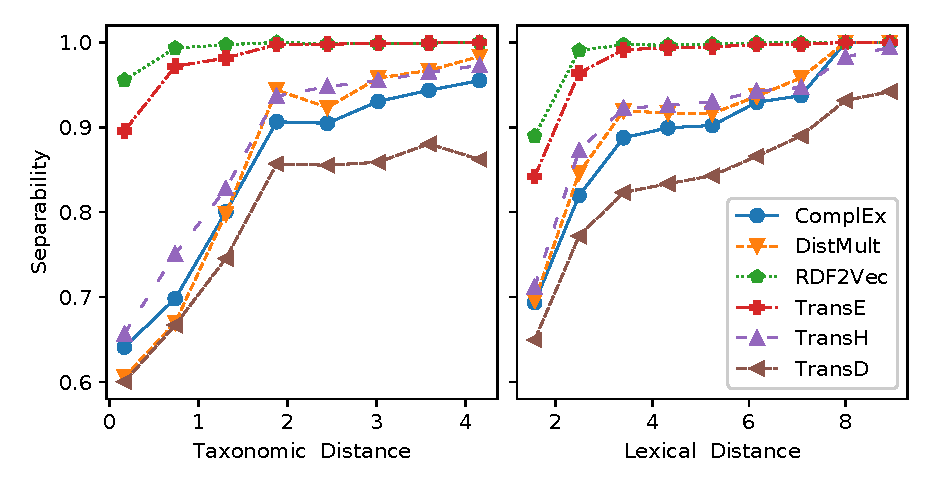
\includegraphics[width=\linewidth]{fig/plot/sep1_dist.eps}
  \caption{Séparabilité moyenne entre deux classes en fonction de leur distance taxonomique (à gauche) et de leur distance lexicale (à droite), pour différents modèles de plongement. }
  \label{fig:separability-lexical}
\end{figure}

\begin{figure}[h]
  \centering
  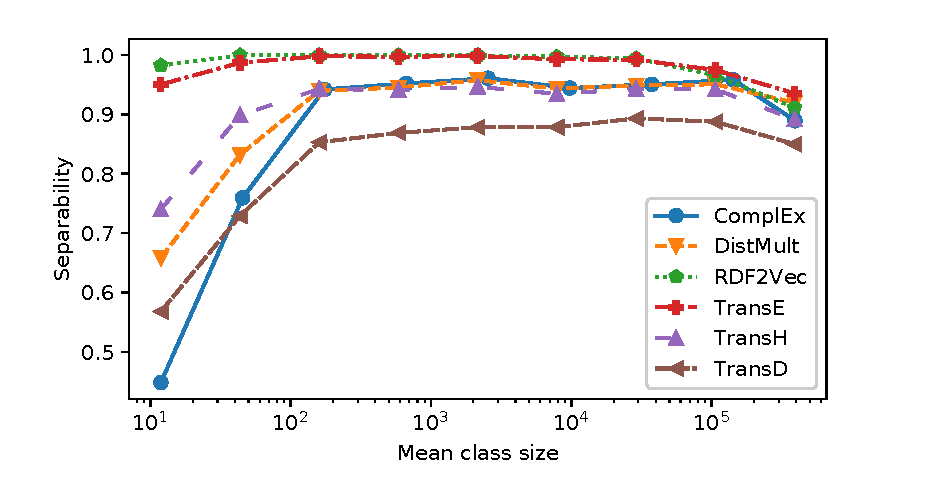
\includegraphics[width=\linewidth]{fig/plot/separability2_type1.eps}
  \caption{Séparabilité moyenne entre deux classes en fonction de la fréquence de ces classes, pour différents modèles de plongement.}
  \label{fig:separability-freq}
\end{figure}

Comme attendu, le score de séparabilité est dépendant de la distance lexicale et taxonomique entre les classes, et ce pour tous les modèles. Tous les modèles sauf TransD parviennent à séparer correctement les classes distantes (distance lexicale supérieur à 8, ou distance taxonomique supérieure à 3); en revanche, seuls deux modèles parviennent à conserver des scores élevés sur l'essentiel de l'intervalle : RDF2Vec et TransE, avec un avantage net pour RDF2Vec dans les faibles distances. La séparabilité moyenne de ces deux modèles diminue pour les classes très proches (distance taxonomique inférieure à 1, distance lexicale inférieure à 2), mais elle demeure supérieure à 85\%. Tous les autres modèles obtiennent des résultats nettement inférieurs.

Dans la figure \ref{fig:separability-freq}, on observe que les classes rares sont plus difficilement séparables que les classes fréquentes, quoique tous les modèles n'ont pas la même sensibilité à la fréquence : RDF2Vec et TransE n'ont qu'une légère baisse de score pour les classes rares (moins de $10^2$ instances en moyenne), qui peut partiellement être causée par le faible nombre d'échantillons sur lesquels entraîner la SVM. En revanche, les autres modèles ComplEx, DistMult, TransH et TransD y sont très sensibles. Cette sensibilité ne s'explique pas par une corrélation entre les paires rares et les paires proches, puisque les coefficients de Spearman et de Pearson entre les variables de distance et de fréquence sont proches de zéro.

%we observe that rare classes are indeed less separable than more frequent classes, with some variability depending on embedding models. RDF2Vec is once again the best model, with TransE slightly behind. TransH, DistMult and ComplEx have close scores in the size range $[200, 10^5]$, but ComplEx is more sensitive to rare classes than DistMult, which is itself more sensitive than TransH. More surprisingly, we observe that scores also decrease for very frequent classes (mean size above $10^5$ instances) for all embedding models. Both Pearson and Spearman’s correlations between lexical distance and mean class size are close to zero, which rules out the possibility of a bias in the dataset. An explanation is that frequent classes are more likely to be parent of other classes in the dataset (for example, \texttt{dbo:Agent} is the second most frequent class of the dataset, and is a parent of half the classes in the DBpedia ontology), and separating a subclass from its parent is harder than separating sibling or unrelated classes. Finally, we observe a convergence of scores for frequent classes between all models, with TransE achieving the highest score.

En résumé, seuls deux modèles obtiennent une mesure $F1$ moyenne supérieure à 95\% sur notre tâche de séparabilité : RDF2Vec et TransE, avec respectivement 99.7\% et 99?2\% respectivement. 
%\label{sec:kge-sep}
